\documentclass[main.tex]{subfiles}

\begin{document}
\begin{center}
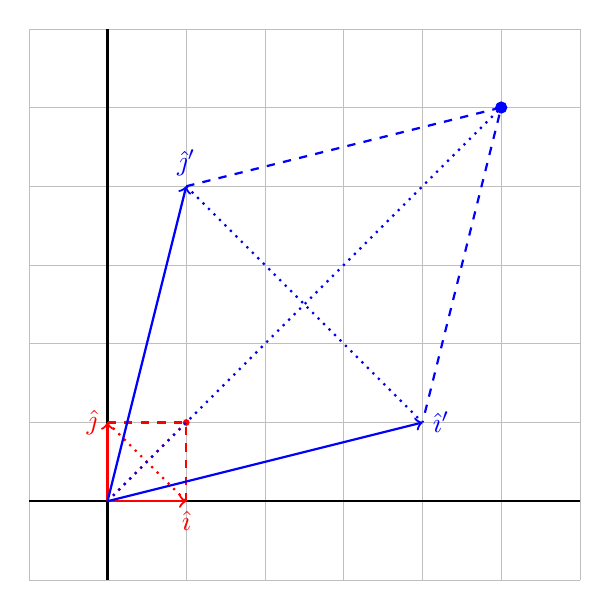
\begin{tikzpicture}
	% Grid and axes.
	\draw[very thin, lightgray] (-1, -1) grid (6, 6);
	\draw[thick, black] (-1, 0) -- (6, 0);
	\draw[thick, black] (0, -1) -- (0, 6);
	% Pre-transformation.
	\draw[->, thick, red] (0, 0) -- (1, 0)
		node[below] {$\hat \imath$};
	\draw[->, thick, red] (0, 0) -- (0, 1)
		node[left] {$\hat \jmath$};
	\draw[dashed, thick, red] (0, 1) -- (1, 1) -- (1, 0);
	\draw[dotted, thick, red] (0, 1) -- (1, 0);
	\draw[dotted, thick, red] (0, 0) -- (1, 1);
	\filldraw[red] (1, 1) circle (1 pt);
	% Post-transformation.
	\draw[->, thick, blue] (0, 0) -- (4, 1)
		node[right] {$\hat \imath^\prime$};
	\draw[->, thick, blue] (0, 0) -- (1, 4)
		node[above] {$\hat \jmath^\prime$};
	\draw[dashed, thick, blue] (1, 4) -- (5, 5) -- (4, 1);
	\draw[dotted, thick, blue] (1, 4) -- (4, 1);
	\draw[dotted, thick, blue] (0, 0) -- (5, 5);
	\filldraw[blue] (5, 5) circle (2 pt);
\end{tikzpicture}
\end{center}
\end{document}